\begin{figure}[tbp]
\centering
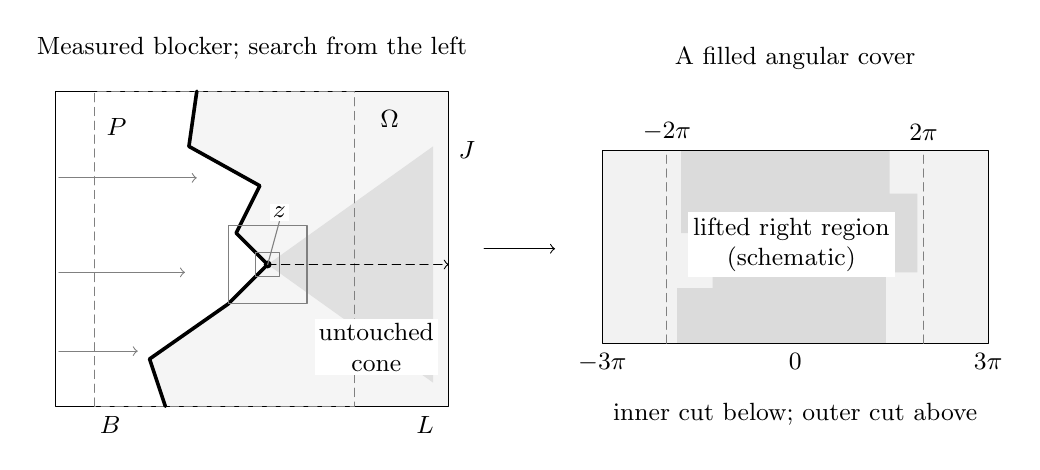
\begin{tikzpicture}[x=1cm,y=1cm,font=\small,line cap=round,line join=round]
  \path[fill=gray!8] (1.4,0) -- (1.2,.6) -- (2.2,1.3) -- (2.7,1.8) -- (2.3,2.2)
    -- (2.6,2.8) -- (1.7,3.3) -- (1.8,4) -- (5,4) -- (5,0) -- cycle;
  \path[fill=gray!24] (2.7,1.8) -- (4.8,.3) -- (4.8,3.3) -- cycle;
  \draw (0,0) rectangle (5,4);
  \draw[gray,densely dashed] (.5,0) rectangle (3.8,4);
  \draw[line width=1.3pt] (1.4,0) -- (1.2,.6) -- (2.2,1.3) -- (2.7,1.8) -- (2.3,2.2)
    -- (2.6,2.8) -- (1.7,3.3) -- (1.8,4);
  \draw[->,gray] (.05,.7) -- (1.05,.7);
  \draw[->,gray] (.05,1.7) -- (1.65,1.7);
  \draw[->,gray] (.05,2.9) -- (1.8,2.9);
  \draw[densely dashed,->] (2.7,1.8) -- (5,1.8);
  \draw[gray] (2.2,1.3) rectangle (3.2,2.3);
  \draw[gray] (2.55,1.65) rectangle (2.85,1.95);
  \fill (2.7,1.8) circle (.05);
  \draw[gray] (2.85,2.35) -- (2.7,1.8);
  \node[above,fill=white,inner sep=1pt] at (2.85,2.35) {$z$};
  \node at (.78,3.55) {$P$};
  \node at (4.25,3.65) {$\Omega$};
  \node[below] at (.7,0) {$B$};
  \node[below] at (4.7,0) {$L$};
  \node[right] at (5,3.25) {$J$};
  \node[fill=white,inner sep=1.5pt,align=center] at (4.08,.75) {untouched\\cone};
  \node[align=center] at (2.5,4.55) {Measured blocker; search from the left};
  \draw[->] (5.45,2) -- (6.35,2);
  \path[fill=gray!10] (6.95,.8) rectangle (11.85,3.25);
  \path[fill=gray!28] (7.9,.8) -- (7.9,1.5) -- (8.35,1.5) -- (8.35,2.2) -- (7.95,2.2)
    -- (7.95,3.25) -- (10.6,3.25) -- (10.6,2.7) -- (10.95,2.7) -- (10.95,1.7)
    -- (10.55,1.7) -- (10.55,.8) -- cycle;
  \draw (6.95,.8) rectangle (11.85,3.25);
  \draw[gray,densely dashed] (7.77,.8) -- (7.77,3.25);
  \draw[gray,densely dashed] (11.03,.8) -- (11.03,3.25);
  \node[below] at (6.95,.8) {$-3\pi$};
  \node[below] at (9.4,.8) {$0$};
  \node[below] at (11.85,.8) {$3\pi$};
  \node[above] at (7.77,3.25) {$-2\pi$};
  \node[above] at (11.03,3.25) {$2\pi$};
  \node[align=center,fill=white,inner sep=2pt] at (9.35,2.05) {lifted right region\\(schematic)};
  \node[above] at (9.4,4.15) {A filled angular cover};
  \node[align=center] at (9.4,-.1) {inner cut below; outer cut above};
\end{tikzpicture}
\caption{The path-defect geometry. The complete complementary-face search leaves the strict right side $\Omega$ of the measured path $P$ uninspected. An exposed vertex $z$ supplies the entire horizontal ray segment from $z$ to the right edge of $L$, with a cone portion contained in that side. After discarding supports hitting the $P$ hub, the annular part lifts to bounded angular coordinates. The pale rectangle on the right represents the larger regular sector used for coefficient transplantation, not an assertion that all of that sector was originally uninspected. External attachments leave through the outlet arc $J$.}
\label{fig:path-defect}
\end{figure}
